% 2010 年天津卷理科第 19 题：长方体 ABCD-A1B1C1D1，E、F 分别在 BC、CC1 上。
% 来源 PDF：普通高考/2010/2010天津理.pdf，SHA-256 340aba76699a12f330637f9c682abbc893e03e0e91788287934c0a7e0a3cace9。
% 原页：第 2 页（A3 六栏）第 1 栏下部，书页码 636。
% 重绘依据：AB:AD:AA1=1:2:4，CF=AB=2CE；可见棱实线，被遮挡的 AB、AD、AA1 虚线；
%   另画平面 A1ED 的 A1E、A1D、ED（虚线）与 AF（虚线）、EF（实线）。
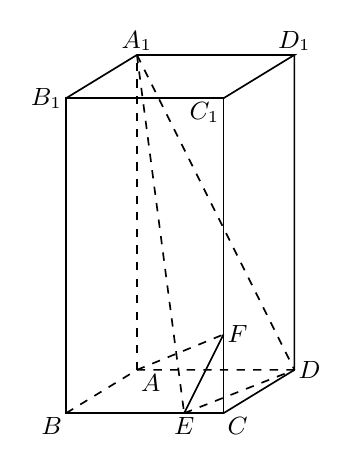
\begin{tikzpicture}[semithick, every node/.style={inner sep=1.2pt, font=\small}]
  \coordinate (B) at (0,0);
  \coordinate (C) at (2,0);
  \coordinate (C1) at (2,4);
  \coordinate (B1) at (0,4);
  \coordinate (A) at (0.9,0.55);
  \coordinate (D) at (2.9,0.55);
  \coordinate (D1) at (2.9,4.55);
  \coordinate (A1) at (0.9,4.55);
  \coordinate (E) at (1.5,0);
  \coordinate (F) at (2,1);
  % 可见棱
  \draw (B) -- (C) -- (C1) -- (B1) -- cycle;
  \draw (B1) -- (A1) -- (D1) -- (C1);
  \draw (D1) -- (D) -- (C);
  % 被遮挡的棱
  \draw[dashed] (B) -- (A) -- (D);
  \draw[dashed] (A) -- (A1);
  % 题设点与辅助线
  \draw (E) -- (F);
  \draw[dashed] (A1) -- (E);
  \draw[dashed] (A1) -- (D);
  \draw[dashed] (E) -- (D);
  \draw[dashed] (A) -- (F);
  \node[above] at (A1) {$A_1$};
  \node[above] at (D1) {$D_1$};
  \node[left] at (B1) {$B_1$};
  \node[below left] at (C1) {$C_1$};
  \node[below left] at (B) {$B$};
  \node[below right] at (C) {$C$};
  \node[right] at (D) {$D$};
  \node[below right] at (A) {$A$};
  \node[below] at (E) {$E$};
  \node[right] at (F) {$F$};
\end{tikzpicture}
